% Name: D flip-flop timing
% Description: A rising-edge D flip-flop and its timing diagram: Q takes the value of D at each rising clock edge and ignores the brief pulse on D between edges.
% Tags: D flip-flop, timing diagram, clock, sequential logic

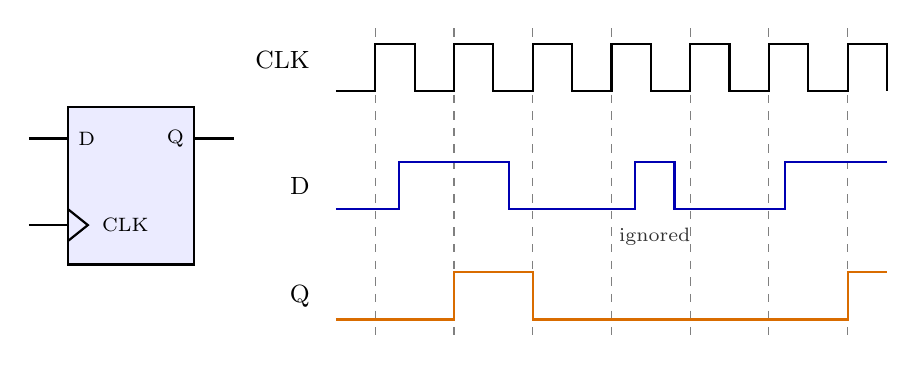
\begin{tikzpicture}[thick, every node/.style={font=\small}]
  % The flip-flop symbol, with the clock input's triangle
  \draw[fill=blue!8] (-3.4,-2.6) rectangle (-1.8,-0.6);
  \draw (-3.4,-2.3) -- (-3.15,-2.1) -- (-3.4,-1.9);
  \node[anchor=west, font=\scriptsize] at (-3.4,-1) {D};
  \node[anchor=west, font=\scriptsize] at (-3.1,-2.1) {CLK};
  \node[anchor=east, font=\scriptsize] at (-1.8,-1) {Q};
  \draw (-3.9,-1) -- (-3.4,-1) (-3.9,-2.1) -- (-3.4,-2.1) (-1.8,-1) -- (-1.3,-1);
  % Rising clock edges at t = 0.5, 1.5, ..., 6.5; Q copies D there: 0, 1, 0, 0, 0, 0, 1
  \foreach \t in {0.5,1.5,...,6.5} \draw[thin, dashed, gray] (\t,0.4) -- (\t,-3.6);
  \node[anchor=east] at (-0.2,0) {CLK};
  \draw (0,-0.4) \foreach \t in {0,1,...,6} { -- (\t,-0.4) -- (\t+0.5,-0.4) -- (\t+0.5,0.2) -- (\t+1,0.2) -- (\t+1,-0.4) };
  \node[anchor=east] at (-0.2,-1.6) {D};
  \draw[blue!70!black] (0,-1.9) -- (0.8,-1.9) -- (0.8,-1.3) -- (2.2,-1.3) -- (2.2,-1.9) -- (3.8,-1.9) -- (3.8,-1.3) -- (4.3,-1.3) -- (4.3,-1.9) -- (5.7,-1.9) -- (5.7,-1.3) -- (7,-1.3);
  \node[anchor=east] at (-0.2,-3) {Q};
  \draw[orange!85!black] (0,-3.3) -- (1.5,-3.3) -- (1.5,-2.7) -- (2.5,-2.7) -- (2.5,-3.3) -- (6.5,-3.3) -- (6.5,-2.7) -- (7,-2.7);
  \node[font=\scriptsize, gray!40!black] at (4.05,-2.25) {ignored};
\end{tikzpicture}
